\documentclass{article}

%\usepackage[nonatbib]{neurips_2020}
\usepackage[preprint]{neurips_2020}
\usepackage[utf8]{inputenc} % allow utf-8 input
\usepackage[T1]{fontenc}    % use 8-bit T1 fonts
\usepackage{hyperref}       % hyperlinks
\usepackage{url}            % simple URL typesetting
\usepackage{booktabs}       % professional-quality tables
\usepackage{amsfonts}       % blackboard math symbols
\usepackage{nicefrac}       % compact symbols for 1/2, etc.
\usepackage{microtype}      % microtypography
\usepackage[nottoc]{tocbibind}
\usepackage{graphicx}
\usepackage{float}
\usepackage[
    backend=biber,
    style=nature,
]{biblatex}
\addbibresource{reference.bib}

\title{Classification of X-ray images using different models}

% The \author macro works with any number of authors. There are two commands
% used to separate the names and addresses of multiple authors: \And and \AND.
%
% Using \And between authors leaves it to LaTeX to determine where to break the
% lines. Using \AND forces a line break at that point. So, if LaTeX puts 3 of 4
% authors names on the first line, and the last on the second line, try using
% \AND instead of \And before the third author name.

\author{
 \textbf{Choi, Moon-ki}\\
 \and
 \textbf{Choi, Won Joon}\\
 \and
 \textbf{Kim, Hyunwoo}\\
    \and
 \textbf{Lee, Garim}\\
}

\begin{document}

\maketitle
% \begin{abstract}
%   The abstract paragraph should be indnted \nicefrac{1}{2}~inch (3~picas) on
%   both the left- and right-hand margins. Use 10~point type, with a vertical
%   spacing (leading) of 11~points.  The word \textbf{Abstract} must be centered,
%   bold, and in point size 12. Two line spaces precede the abstract. The abstract
%   must be limited to one paragraph.
% \end{abstract}
\section{Motivation}

Diagnostic of pneumonia through the chest X-ray image requires significant reliability because a mistake in this process brings hazardous impact on a patient. In this project, our team “lifesaver” will propose several diagnostic tools based on the machine learning model including what we learned from the lecture. Machined learning based diagnostic tools will bring a strong impact on the diagnostic of pneumonia because of three reasons.\\\\
1. Diagnostic tools can quantify the progress the how far pneumonia has progressed and diagnose the type of pneumonia whether it is caused by virus or bacteria
\vspace{2mm}
\\2. The tools can prevent the mistake from the human expert by providing additional features to diagnose the status of the chest of the patient.
\vspace{2mm}
\\3. Because of the convenience and quick test after the tool is settled, It can capture pneumonia from the x-ray image for other patients who intended to take the x-ray image for other diseases. \\\\
Throughout this project, we expect that the machine learning model will be able to diagnose pneumonia and its type quantitatively and which model is appropriate for screening pneumonia among the various models used in this project.


\section{Formalization into data mining task}
Based on the purpose of our project, classification will be conducted to detect pneumonia as a binary classifier. Support vector machine (SVM), deep neural network (DNN), convolutional neural network (CNN), and transfer learning will be used, and evaluation measures will be compared to select the final model.

First, SVM is a widely used supervised learning model for classification that uses linear or nonlinear decision boundaries to separate classes \cite{KUMARBOOK}. It is also known that SVM performs notably in image classification tasks such as image recognition \cite{ROBUST}. Second, in class, we learned that neural networks can be used for challenging areas such as image classification \cite{KUMARBOOK}. Specifically, DNN and CNN were chosen because they were proven to show successful performance in tasks using images, for example,  image classification, object identification, and face recognition. Also, transfer learning allows classification of a new dataset using related pre-trained data. If a model is trained on enough dataset for image classification, the model using transfer learning will show adequate accuracy in classifying another model.

\section {Data Logistics}
The dataset is organized into 3 folders which has train, test, and validation datasets. All dataset contains subfolders for each image category (Pneumonia/Normal). There are 5,863 X-Ray images (JPEG) and 2 categories (Pneumonia/Normal) in total.\\
Chest x-ray images (frontal larynx) were selected as a retrospective cohort for children aged 1 to 5 at Guangzhou Women's and Children's Hospital. All chest X-ray imaging was performed as part of the patient's routine clinical treatment.\\
For the analysis of chest X-ray images, all chest radiographs were initially screened for quality control by eliminating all low-quality or non-readable scans. Then, diagnostic scores on images were scored by two specialists before they were deleted for AI system training. To account for all rating errors, the evaluation set was also confirmed by a third expert.
\cite{PNEUMONIA_IMAGE}. 
    \begin{figure}[H]
        \centering
    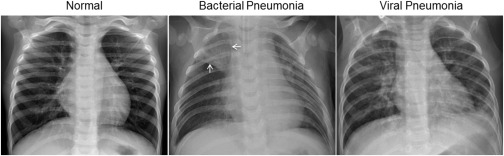
\includegraphics[width=0.7\textwidth]{figures/Pneumonia.jpg}
    \caption{chest X-Ray}
    \end{figure}
    
The normal chest x-ray (left panel) shows clear lungs with no abnormal surgical site in the image. Bacterial pneumonia (middle) typically exhibits focal lobar bonds in the right upper lobe (white arrow), while viral pneumonia (right) exhibits a more diffuse "interval" pattern in both lungs.



\section{Related work}
\textbf{Convolutional neural network(CNN):}\\\\
Convolutional neural network(CNN) has had ground breaking results in the field of Deep Learning. CNN has its strength in pattern recognition such as image classification and voice recognition\cite{8308186}. Artificial neural network(ANN) uses a naive approach of training parameters whereas CNN reduces this complex task in large datasets of the modern world by taking a different route. For example, if the image that we are trying to train on is $32 \times 32$ pixels with 3 RGB channels, there would be $32 \times 32 \times 3$ with only one neuron. By adding more neurons and layers, parameters that will be updated become very large which takes a considerable amount of time. Convolution reduces complexity by taking a portion of the image per neuron. We will discuss more about the process of the convolutional neural network further in this project.
\\\\
\textbf{Using deep learning algorithm  for detecting pneumonia from X-rays:}\\\\
Our project focuses on the classification of pneumonia X-rays images. This article experiments using the convolutional neural network with the rectified linear unit(ReLU) as the activation function and Adam optimization function to test the result\cite{sagar_2019}. 
    \begin{figure}[H]
        \centering
    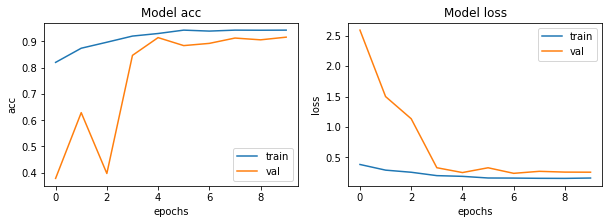
\includegraphics[width=0.7\textwidth]{figures/article_accuracy_loss.png}
    \caption{Credit: Abhinav Sagar}
    \end{figure}
As we can see from the figure, model accuracy and loss improves within 10 epochs. The model achieves 90\% accuracy on the validation set which can be improved as the model is further trained. In this project, we will use various algorithms to compare the results and discuss the tradeoffs among the models created.
\printbibliography
%\bibliographystyle{abbrv}
%\bibliography{reference}
\end{document}